\documentclass[11pt,a4paper]{article}
\usepackage[margin=16mm,top=49mm,bottom=19mm,headheight=34mm,headsep=5mm]{geometry}
\usepackage{fontspec}
\setmainfont{Times New Roman}
\usepackage{amsmath,amssymb}
\usepackage{graphicx,array,longtable}
\usepackage[table]{xcolor}
\usepackage{fancyhdr}
\usepackage[hidelinks]{hyperref}
\hypersetup{pdftitle={Program Remedial dan Pengayaan Matematika Fase F XI - Transformasi Fungsi},pdfauthor={Nurmadinah, S.Pd.}}
\setlength{\parindent}{0pt}
\setlength{\LTpre}{3pt}\setlength{\LTpost}{4pt}
\setlength{\emergencystretch}{2em}
\linespread{1.08}
\pagestyle{fancy}\fancyhf{}
\renewcommand{\headrulewidth}{0pt}
\fancyhead[C]{\begin{minipage}{\textwidth}
\noindent\begin{minipage}[c]{23mm}
\centering
\includegraphics[width=20mm,height=23mm,keepaspectratio]{logo.png}
\end{minipage}%
\begin{minipage}[c]{132mm}\centering
{\fontsize{10.2}{12}\selectfont\bfseries KEMENTERIAN AGAMA REPUBLIK INDONESIA\\
KANTOR KEMENTERIAN AGAMA KABUPATEN GOWA}\\[2pt]
{\fontsize{13}{15}\selectfont\bfseries MAN INSAN CENDEKIA GOWA}\\[2pt]
{\fontsize{8.3}{10.5}\selectfont
\mbox{Jl. Pendidikan Desa Belapunrangan, Kec. Parangloe, Gowa, Sulawesi Selatan 92173}\\
\mbox{Telp. 085173279846 $\cdot$ Pos-el: insancendekiagowa@gmail.com $\cdot$ Laman: icgowa.sch.id}}
\end{minipage}%
\begin{minipage}[c]{23mm}\strut\end{minipage}
\par\vspace{2mm}\hrule height1.2pt\vspace{1.2pt}\hrule height.4pt
\end{minipage}}
\fancyfoot[L]{\fontsize{8}{10}\selectfont Program Remedial dan Pengayaan Matematika $|$ Nurmadinah, S.Pd.}
\fancyfoot[R]{\fontsize{8}{10}\selectfont\thepage}
\begin{document}
\begin{center}\bfseries\large PROGRAM REMEDIAL DAN PENGAYAAN\\[2pt] MATEMATIKA FASE F KELAS XI\\[2pt] MATERI TRANSFORMASI FUNGSI\end{center}\medskip
\begin{center}TAHUN PELAJARAN 2026/2027\end{center}
\vspace{19.84251969pt}
{\small\setlength{\tabcolsep}{2mm}\renewcommand{\arraystretch}{1.35}\begin{longtable}{|>{\raggedright\arraybackslash}p{49.324mm}|>{\raggedright\arraybackslash}p{120.226mm}|}\hline
Satuan pendidikan & MAN Insan Cendekia Gowa\\ \hline
Mata pelajaran & Matematika\\ \hline
Fase / kelas & F / XI\\ \hline
Elemen & Aljabar dan Fungsi\\ \hline
Materi & Transformasi Fungsi\\ \hline
Guru penyusun & Nurmadinah, S.Pd.\\ \hline
NIP & 199402222020122022\\ \hline
Semester & Ganjil\\ \hline
Alokasi rencana & Remedial: 6 JP; pengayaan: 4 JP. Satu JP direncanakan 45 menit. Penjadwalan mengikuti kebutuhan peserta dan program madrasah.\\ \hline
\end{longtable}}\medskip
\vspace{8mm}\noindent\begin{minipage}[t]{.61\linewidth}Mengetahui,\\Kepala Madrasah,\\[22mm]Dr. Burhanuddin, S.Ag., M.Fil.I.\\NIP 197609152007101001\end{minipage}\hfill\begin{minipage}[t]{.35\linewidth}Gowa, 13 Juli 2026\\Guru Mata Pelajaran,\\[22mm]\textbf{Nurmadinah, S.Pd.}\\NIP 199402222020122022\end{minipage}
\clearpage
\begin{center}\bfseries\large A. LANDASAN DAN TUJUAN PROGRAM\end{center}\medskip
{\small\setlength{\tabcolsep}{2mm}\renewcommand{\arraystretch}{1.35}\begin{longtable}{|>{\raggedright\arraybackslash}p{60.554mm}|>{\raggedright\arraybackslash}p{108.996mm}|}\hline
\rowcolor{gray!10}\textbf{Acuan} & \textbf{Arah penerapan}\\ \hline
\endfirsthead
\rowcolor{gray!10}\textbf{Acuan} & \textbf{Arah penerapan}\\ \hline
\endhead
KMA 450 Tahun 2024 sebagaimana diubah dengan KMA 1503 Tahun 2025 & Layanan belajar sesuai kebutuhan murid dan penguatan nilai cinta ilmu, saling membantu, serta kepedulian lingkungan. [1]\\ \hline
Permendikdasmen 13 Tahun 2025 dan 1 Tahun 2026 & Kerangka kurikulum serta standar proses untuk perencanaan, pelaksanaan, dan penilaian proses. [2][3]\\ \hline
Permendikbudristek 21 Tahun 2022 & Bukti belajar digunakan untuk menilai kemajuan secara objektif dan menentukan tindak lanjut. [4]\\ \hline
Keputusan Kepala BSKAP 046/H/KR/2025 & CP Matematika Fase F, elemen Aljabar dan Fungsi. [5]\\ \hline
Panduan Pembelajaran dan Asesmen, revisi 2025 & Asesmen formatif, pendampingan pada kompetensi yang belum dikuasai, serta pengayaan untuk pendalaman. [6]\\ \hline
\end{longtable}}\medskip
\par\medskip\noindent\textbf{Capaian Pembelajaran yang relevan}\par\smallskip
“Menentukan fungsi invers, komposisi fungsi, dan transformasi fungsi untuk memodelkan situasi dunia nyata menggunakan fungsi yang sesuai (linear, kuadrat, eksponensial).” [5]\par\medskip
{\small Penjelasan resmi Kemendikdasmen tanggal 23 Juni 2026 menyatakan perubahan CP melalui Keputusan Kepala BKPDM Nomor 020 Tahun 2026 hanya mencakup Agama dan Budi Pekerti. CP Matematika tetap menggunakan keputusan tahun 2025. [7]\par}\medskip
\par\medskip\noindent\textbf{Tujuan program}\par\smallskip
Program membantu murid menghubungkan perubahan rumus dengan perubahan grafik, memperbaiki miskonsepsi arah translasi dan faktor skala, serta memodelkan situasi melalui transformasi fungsi linear, kuadrat, dan eksponensial. Penempatan materi di kelas XI diselaraskan dengan ATP madrasah; CP merupakan target akhir fase.\par\medskip
{\small Program memuat rencana dan instrumen. Nama peserta, tanggal pelaksanaan, level awal/akhir, serta hasil program dicatat setelah kegiatan berdasarkan bukti nyata.\par}\medskip
\clearpage
\begin{center}\bfseries\large B. TUJUAN PEMBELAJARAN DAN KKTP\end{center}\medskip
{\small\setlength{\tabcolsep}{2mm}\renewcommand{\arraystretch}{1.35}\begin{longtable}{|>{\raggedright\arraybackslash}p{16.269mm}|>{\raggedright\arraybackslash}p{67.787mm}|>{\raggedright\arraybackslash}p{81.344mm}|}\hline
\rowcolor{gray!10}\textbf{Kode} & \textbf{Tujuan pembelajaran} & \textbf{Bukti esensial ketercapaian}\\ \hline
\endfirsthead
\rowcolor{gray!10}\textbf{Kode} & \textbf{Tujuan pembelajaran} & \textbf{Bukti esensial ketercapaian}\\ \hline
\endhead
TP1 & Membaca grafik dasar fungsi linear, kuadrat, dan eksponensial. & Menentukan minimal tiga titik, titik acuan, domain dan range pada konteks yang diberikan.\\ \hline
TP2 & Menentukan translasi horizontal dan vertikal suatu fungsi. & Menggunakan rumus pergeseran dengan tanda yang tepat serta memeriksa minimal dua titik.\\ \hline
TP3 & Menganalisis refleksi grafik terhadap sumbu koordinat. & Membedakan perubahan keluaran dan masukan; memeriksa pasangan titik sebelum dan sesudah refleksi.\\ \hline
TP4 & Menentukan peregangan/pemampatan vertikal dan horizontal. & Menentukan faktor skala geometris dengan benar dan menjelaskan perbedaan pengali di luar dan di dalam fungsi.\\ \hline
TP5 & Menyusun urutan transformasi dan menafsirkan modelnya. & Memperoleh rumus dan titik acuan yang benar, menjelaskan urutan operasi, serta menafsirkan domain, satuan, dan batas model.\\ \hline
\end{longtable}}\medskip
\par\medskip\noindent\textbf{Rubrik ketercapaian per tujuan}\par\smallskip
{\small\setlength{\tabcolsep}{2mm}\renewcommand{\arraystretch}{1.35}\begin{longtable}{|>{\raggedright\arraybackslash}p{41.693mm}|>{\raggedright\arraybackslash}p{127.857mm}|}\hline
\rowcolor{gray!10}\textbf{Level} & \textbf{Deskripsi operasional}\\ \hline
\endfirsthead
\rowcolor{gray!10}\textbf{Level} & \textbf{Deskripsi operasional}\\ \hline
\endhead
1 - Perlu dukungan intensif & Belum menunjukkan konsep utama walaupun diberi pertanyaan penuntun.\\ \hline
2 - Berkembang & Sebagian langkah tepat; masih terdapat kesalahan konsep atau membutuhkan arahan pada langkah utama.\\ \hline
3 - Tercapai & Seluruh bukti esensial TP tampak secara mandiri, dengan hasil dan penjelasan yang dapat diperiksa.\\ \hline
4 - Melampaui & Memenuhi level 3 serta memberi pemeriksaan berbeda, contoh pembanding, atau generalisasi yang sah.\\ \hline
\end{longtable}}\medskip
{\small KKTP program: setiap TP ditargetkan minimal level 3. TP level 1-2 diberi remedial terarah; TP yang telah tercapai dapat diberi pengayaan. Level dan kriteria ini merupakan rancangan guru untuk unit, bukan ambang nilai nasional. Penilaian tidak hanya berdasarkan total jawaban benar.\par}\medskip
\clearpage
\begin{center}\bfseries\large C. PETA KONSEP DAN MEDIA PENDAMPING\end{center}\medskip
{\small\setlength{\tabcolsep}{2mm}\renewcommand{\arraystretch}{1.35}\begin{longtable}{|>{\raggedright\arraybackslash}p{29.624mm}|>{\raggedright\arraybackslash}p{54.310mm}|>{\raggedright\arraybackslash}p{81.466mm}|}\hline
\rowcolor{gray!10}\textbf{Transformasi} & \textbf{Rumus hasil} & \textbf{Pemetaan titik / makna}\\ \hline
\endfirsthead
\rowcolor{gray!10}\textbf{Transformasi} & \textbf{Rumus hasil} & \textbf{Pemetaan titik / makna}\\ \hline
\endhead
Translasi & \(g(x)=f(x-h)+k\) & \((u,v)\mapsto(u+h,v+k)\). Positif \(h\): ke kanan; positif \(k\): ke atas.\\ \hline
Refleksi sumbu x & \(g(x)=-f(x)\) & \((u,v)\mapsto(u,-v)\).\\ \hline
Refleksi sumbu y & \(g(x)=f(-x)\) & \((u,v)\mapsto(-u,v)\). Pada fungsi genap, grafik dapat tetap sama.\\ \hline
Skala vertikal & \(g(x)=af(x)\), \(a\ne0\) & \((u,v)\mapsto(u,av)\). Faktor geometris \(|a|\); jika \(a<0\), disertai refleksi sumbu x.\\ \hline
Skala horizontal & \(g(x)=f(bx)\), \(b\ne0\) & \((u,v)\mapsto\left(\frac{u}{b},v\right)\). Faktor geometris \(\frac1{|b|}\); jika \(b<0\), disertai refleksi sumbu y.\\ \hline
Gabungan & \(g(x)=af\bigl(b(x-h)\bigr)+k\) & \((u,v)\mapsto\left(h+\frac{u}{b},k+av\right)\); \(a,b\ne0\). Pemetaan membantu memeriksa hasil.\\ \hline
\end{longtable}}\medskip
\begin{center}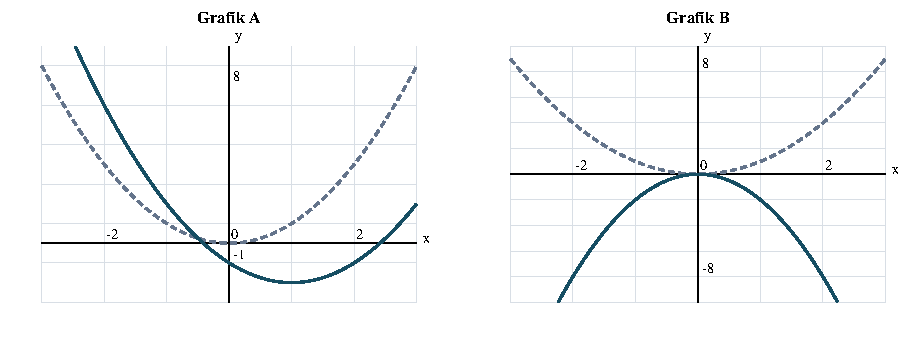
\includegraphics[width=\linewidth,height=62mm,keepaspectratio]{grafik.pdf}\end{center}
{\small Garis putus-putus: \(f(x)=x^2\). Garis penuh grafik A: \(g(x)=(x-1)^2-2\); grafik B: \(g(x)=-2x^2\). Bandingkan titik acuan dan faktor skala.\par}\medskip
\clearpage
\begin{center}\bfseries\large LAMPIRAN 1. ASESMEN AWAL\end{center}\medskip
{\small Nama: \_\_\_\_\_\_\_\_\_\_\_\_\_\_\_\_\_\_\_\_\_\_\_\_\_\_\_\_\_\_\_\_\_\_  Kelas: \_\_\_\_\_\_\_\_\_\_\par}\medskip
{\small Waktu rencana: 30 menit. Kerjakan mandiri dan jelaskan alasan. Gunakan kertas berpetak bila diperlukan.\par}\medskip
\noindent\textbf{D1 / TP1.} Lengkapi nilai \(x=-1,0,1\) untuk \(f(x)=2x+1\), \(p(x)=x^2\), dan \(q(x)=2^x\). Tentukan domain dan range masing-masing jika domain asalnya seluruh bilangan real.\par\vspace{10mm}
\noindent\textbf{D2 / TP2.} Dari \(f(x)=x^2\) diperoleh \(g(x)=(x-2)^2+3\). Jelaskan pergeseran, tentukan titik puncak, serta periksa \(g(1)\) dan \(g(3)\).\par\vspace{10mm}
\noindent\textbf{D3 / TP3.} Untuk \(f(x)=2^x\), tulis rumus hasil refleksi terhadap sumbu x dan terhadap sumbu y. Tentukan pasangan titik bayangan dari \((1,2)\) pada masing-masing refleksi.\par\vspace{10mm}
\noindent\textbf{D4 / TP4.} Diketahui \(f(x)=x^2\). Bandingkan \(g(x)=2f(x)\) dengan \(h(x)=f(2x)\). Tentukan faktor skala geometrisnya, bayangan titik \((1,1)\), dan nilai \(g(1)\) serta \(h(1)\).\par\vspace{10mm}
\noindent\textbf{D5 / TP5.} Grafik \(f(x)=x^2\) direfleksikan terhadap sumbu x, lalu digeser 1 satuan ke kanan dan 4 ke atas. Tentukan rumus hasil, titik puncak, dan range-nya. Jelaskan urutan operasi.\par\vspace{10mm}
{\small Guru menilai setiap TP dengan rubrik, kemudian mengonfirmasi alasan melalui wawancara singkat jika jawaban tertulis belum cukup.\par}\medskip
\clearpage
\begin{center}\bfseries\large D. RENCANA PROGRAM REMEDIAL\end{center}\medskip
Peserta dipilih berdasarkan TP level 1-2, bukan pelabelan kemampuan tetap. Satu siklus direncanakan 3 pertemuan × 2 JP. Guru memilih sesi sesuai kebutuhan dan menyesuaikan durasi dengan kemajuan murid.\par\medskip
{\small\setlength{\tabcolsep}{2mm}\renewcommand{\arraystretch}{1.35}\begin{longtable}{|>{\raggedright\arraybackslash}p{16.847mm}|>{\raggedright\arraybackslash}p{89.049mm}|>{\raggedright\arraybackslash}p{16.847mm}|>{\raggedright\arraybackslash}p{38.507mm}|}\hline
\rowcolor{gray!10}\textbf{Sesi} & \textbf{Kegiatan pendampingan} & \textbf{Waktu} & \textbf{Bukti kemajuan}\\ \hline
\endfirsthead
\rowcolor{gray!10}\textbf{Sesi} & \textbf{Kegiatan pendampingan} & \textbf{Waktu} & \textbf{Bukti kemajuan}\\ \hline
\endhead
R1\newline TP1-TP2 & Memahami: wawancara kesalahan dan grafik dasar (15 menit). Mengaplikasi: tabel titik dan kartu pergeseran (35 menit), latihan terbimbing lalu mandiri (30 menit). Merefleksi: tiket keluar tentang tanda pergeseran (10 menit). & 2 JP\newline 90 menit & Tabel, titik puncak, dan dua titik pemeriksaan benar; bantuan dikurangi secara bertahap.\\ \hline
R2\newline TP3-TP4 & Memahami: bedakan masukan dan keluaran (15 menit). Mengaplikasi: pasangkan titik refleksi (25 menit), bandingkan skala vertikal dan horizontal (40 menit). Merefleksi: jelaskan satu miskonsepsi yang diperbaiki (10 menit). & 2 JP\newline 90 menit & Murid menjelaskan faktor kebalikan pada skala horizontal dan memeriksa hasil sendiri.\\ \hline
R3\newline TP5 & Memahami: urutan transformasi dengan kartu proses (15 menit). Mengaplikasi: latihan model dan pemetaan titik (20 menit), asesmen ulang TP sasaran (40 menit). Merefleksi: umpan balik individual dan tindak lanjut (15 menit). & 2 JP\newline 90 menit & Bukti level terbaru dibandingkan dengan awal; TP yang belum tercapai diberi bantuan lanjutan.\\ \hline
\end{longtable}}\medskip
\par\medskip\noindent\textbf{Pelaksanaan yang mendukung murid}\par\smallskip
Gunakan kertas berpetak atau aplikasi grafik bila tersedia. Guru memberikan contoh terurai, mengajak murid menyebutkan alasan, lalu mengurangi bantuan. Tutor sebaya mendukung diskusi dan tidak menggantikan peran guru. Sediakan instruksi terbaca, waktu tambahan, atau jawaban lisan sesuai kebutuhan.\par\medskip
{\small Cinta ilmu dibiasakan melalui pemeriksaan jawaban yang jujur; cinta diri dan sesama melalui bantuan tanpa mempermalukan kesalahan. Tugas konteks lingkungan mendorong kepedulian pada penggunaan sumber daya.\par}\medskip
\par\medskip\noindent\textbf{Keputusan setelah layanan}\par\smallskip
TP minimal level 3 dinyatakan tercapai. Jika belum, ubah bentuk bantuan dan laksanakan siklus singkat berikutnya. Simpan bukti awal, lembar kerja, asesmen ulang, dan umpan balik. Pengolahan nilai mengikuti kebijakan madrasah; program ini tidak menetapkan pembatasan otomatis nilai remedial.\par\medskip
\clearpage
\begin{center}\bfseries\large LAMPIRAN 2. LEMBAR KERJA REMEDIAL\end{center}\medskip
{\small Nama: \_\_\_\_\_\_\_\_\_\_\_\_\_\_\_\_\_\_\_\_\_\_\_\_\_\_\_\_\_\_\_\_\_\_  Kelas: \_\_\_\_\_\_\_\_\_\_\par}\medskip
{\small Guru memilih butir sesuai TP sasaran. Gunakan grafik dasar, pemetaan titik, dan pemeriksaan minimal dua titik.\par}\medskip
\noindent\textbf{R1 / TP1.} Buat tabel \(x=-1,0,1\) untuk \(f(x)=x+2\), \(p(x)=x^2\), dan \(q(x)=2^x\). Bandingkan bentuk grafik, domain, dan range saat fungsi dipandang pada domain real.\par\vspace{9mm}
\noindent\textbf{R2 / TP2.} Untuk \(f(x)=x^2\), tentukan rumus setelah pergeseran 1 ke kiri dan 2 ke bawah. Tuliskan puncak dan bayangan titik \((0,0)\) serta \((1,1)\). Bantuan: perubahan horizontal ditempatkan pada masukan fungsi.\par\vspace{9mm}
\noindent\textbf{R3 / TP3.} Untuk \(f(x)=2^x\), tulis \(-f(x)\) dan \(f(-x)\). Cari bayangan \((1,2)\) dan hitung nilai kedua fungsi saat \(x=1\). Mengapa arah pantulnya berbeda?\par\vspace{9mm}
\noindent\textbf{R4 / TP4.} Bandingkan \(g(x)=3f(x)\) dan \(h(x)=f(3x)\) untuk \(f(x)=x^2\). Tuliskan rumus, faktor skala geometris, serta bayangan titik \((1,1)\) untuk masing-masing.\par\vspace{9mm}
\noindent\textbf{R5 / TP5.} Bentuk \(g(x)=-2f(x-1)+3\) dari \(f(x)=x^2\). Jelaskan satu urutan transformasi yang sesuai, tentukan puncak, range, serta \(g(0)\) dan \(g(2)\).\par\vspace{9mm}
{\small Kesalahan yang saya perbaiki: \_\_\_\_\_\_\_\_\_\_\_\_\_\_\_\_\_\_\_\_\_\_\_\_\_\_\_\_\_\_\_\_\_\_\_\_\_\_\_\_\newline Cara memeriksa hasil saya: \_\_\_\_\_\_\_\_\_\_\_\_\_\_\_\_\_\_\_\_\_\_\_\_\_\_\_\_\_\_\_\_\_\_\_\_\_\_\_\_\_\_\_\par}\medskip
\clearpage
\begin{center}\bfseries\large LAMPIRAN 3. ASESMEN ULANG\end{center}\medskip
{\small Nama: \_\_\_\_\_\_\_\_\_\_\_\_\_\_\_\_\_\_\_\_\_\_\_\_\_\_\_\_\_\_\_\_\_\_  Kelas: \_\_\_\_\_\_\_\_\_\_\par}\medskip
{\small Waktu rencana: 40 menit. Kerjakan mandiri; guru menilai TP yang menjadi sasaran remedial.\par}\medskip
\noindent\textbf{U1 / TP1.} Buat tabel \(x=-1,0,1\) untuk \(f(x)=3x-1\), \(p(x)=x^2\), dan \(q(x)=3^x\). Tentukan domain dan range pada domain real.\par\vspace{9mm}
\noindent\textbf{U2 / TP2.} Grafik \(f(x)=x^2\) digeser 3 ke kanan dan 1 ke bawah. Tentukan rumus, puncak, serta nilai fungsi hasil saat \(x=2\) dan \(x=4\).\par\vspace{9mm}
\noindent\textbf{U3 / TP3.} Untuk \(f(x)=3^x\), tentukan hasil refleksi terhadap sumbu x dan sumbu y. Tuliskan bayangan titik \((1,3)\) dan nilai kedua fungsi hasil saat \(x=1\).\par\vspace{9mm}
\noindent\textbf{U4 / TP4.} Untuk \(f(x)=x^2\), tentukan rumus, faktor skala geometris, dan bayangan titik \((1,1)\) pada \(g(x)=\frac12 f(x)\) dan \(h(x)=f\left(\frac{x}{2}\right)\).\par\vspace{9mm}
\noindent\textbf{U5 / TP5.} Grafik \(f(x)=x^2\) mengalami skala vertikal faktor 2, kemudian refleksi terhadap sumbu x, translasi 2 ke kanan dan 5 ke atas. Tentukan rumus, puncak, range, serta nilai fungsi hasil saat \(x=1\) dan \(x=3\).\par\vspace{9mm}
{\small Gunakan rubrik bagian B. TP tercapai ketika seluruh bukti esensialnya tampak mandiri pada level 3. Periksa konsep dan alasan; kelebihan pada TP lain tidak menggantikan bukti TP yang belum tercapai.\par}\medskip
\clearpage
\begin{center}\bfseries\large E. RENCANA PROGRAM PENGAYAAN\end{center}\medskip
Peserta telah mencapai minimal level 3 pada TP sasaran. Tugas dipilih sesuai minat; murid dapat mendapat pengayaan pada TP yang dikuasai sambil menyelesaikan remedial TP lain.\par\medskip
{\small\setlength{\tabcolsep}{2mm}\renewcommand{\arraystretch}{1.35}\begin{longtable}{|>{\raggedright\arraybackslash}p{15.752mm}|>{\raggedright\arraybackslash}p{112.892mm}|>{\raggedright\arraybackslash}p{36.756mm}|}\hline
\rowcolor{gray!10}\textbf{Sesi} & \textbf{Aktivitas} & \textbf{Waktu / produk}\\ \hline
\endfirsthead
\rowcolor{gray!10}\textbf{Sesi} & \textbf{Aktivitas} & \textbf{Waktu / produk}\\ \hline
\endhead
P1 & Memahami konteks dan memilih tugas (15 menit); mengeksplorasi rumus, grafik, serta pemetaan titik (60 menit); merefleksi asumsi dan memeriksa hasil (15 menit). & 2 JP / 90 menit\newline Draf model, tabel, dan grafik.\\ \hline
P2 & Memperbaiki solusi berdasarkan umpan balik (35 menit); presentasi dan verifikasi individual (35 menit); refleksi keterbatasan serta rencana validasi (20 menit). & 2 JP / 90 menit\newline Laporan 1-2 halaman dan penjelasan individual.\\ \hline
\end{longtable}}\medskip
\par\medskip\noindent\textbf{Proyek A - Apakah urutan transformasi berpengaruh?}\par\smallskip
Definisikan operator \(T(f)(x)=f(x-2)\) dan \(D(f)(x)=2f(x)\). Untuk fungsi \(f(x)=x^2\), bandingkan \(D(T(f))\) dan \(T(D(f))\) melalui rumus serta minimal tiga titik. Selanjutnya definisikan \(V(f)(x)=f(x)+3\); bandingkan \(D(V(f))\) dan \(V(D(f))\).\par\medskip
Tugas: buat tabel/grafik; nyatakan pasangan operasi yang dapat dipertukarkan dan yang tidak; jelaskan alasan; periksa apakah hasil tersebut berlaku untuk fungsi lain dengan satu argumen umum. Hasil diskusi dipertanggungjawabkan masing-masing murid.\par\medskip
\par\medskip\noindent\textbf{Proyek B - Transformasi model penghematan kertas}\par\smallskip
Model awal \(P(t)=100\left(\frac12\right)^t\) lembar per pekan untuk \(t\ge0\). Program baru dimulai pada pekan ke-1 dan dimodelkan \(Q(t)=100\left(\frac12\right)^{2(t-1)}\) untuk \(t\ge1\). Seluruh angka merupakan data simulasi.\par\medskip
Tugas: nyatakan \(Q\) sebagai transformasi \(P\); gunakan pemetaan titik untuk menentukan faktor skala dan pergeseran; hitung \(Q(1)\), \(Q(2)\), \(Q(3)\); tentukan waktu real saat \(Q(t)=25\). Jelaskan pembatasan domain, keterbatasan nilai lembar pecahan, serta cara memeriksa model dengan pengamatan nyata tanpa mengarang data.\par\medskip
\clearpage
\begin{center}\bfseries\large F. RUBRIK PENGAYAAN DAN REFLEKSI\end{center}\medskip
{\small\setlength{\tabcolsep}{2mm}\renewcommand{\arraystretch}{1.35}\begin{longtable}{|>{\raggedright\arraybackslash}p{27.873mm}|>{\raggedright\arraybackslash}p{26.606mm}|>{\raggedright\arraybackslash}p{29.140mm}|>{\raggedright\arraybackslash}p{35.474mm}|>{\raggedright\arraybackslash}p{38.008mm}|}\hline
\rowcolor{gray!10}\textbf{Aspek} & \textbf{Level 1} & \textbf{Level 2} & \textbf{Level 3} & \textbf{Level 4}\\ \hline
\endfirsthead
\rowcolor{gray!10}\textbf{Aspek} & \textbf{Level 1} & \textbf{Level 2} & \textbf{Level 3} & \textbf{Level 4}\\ \hline
\endhead
Model dan grafik & Rumus atau titik acuan belum sesuai. & Sebagian tepat; ada kesalahan tanda atau skala. & Rumus, domain dan titik acuan benar. & Menguji batas atau memberi representasi alternatif yang sah.\\ \hline
Argumen transformasi & Belum dapat memberi urutan. & Urutan dijelaskan dengan arahan. & Urutan dan faktor skala dijelaskan mandiri. & Memberi generalisasi atau contoh penyangkal yang valid.\\ \hline
Evaluasi hasil & Tidak memeriksa kewajaran. & Pemeriksaan terbatas pada hasil akhir. & Memeriksa titik/rumus serta menyebut asumsi. & Menguji keterbatasan dan memberi rencana validasi.\\ \hline
Komunikasi individual & Belum menjelaskan kontribusi. & Bergantung pada jawaban pasangan. & Menjelaskan alasan dan kontribusinya sendiri. & Menanggapi sanggahan serta memperbaiki penjelasan.\\ \hline
\end{longtable}}\medskip
{\small Target: minimal level 3 pada keempat aspek. Ketentuan ini ditetapkan guru untuk tugas pengayaan. Produk kelompok dilengkapi verifikasi individual; kerja sama diberi umpan balik dan tidak menggantikan bukti kompetensi matematika.\par}\medskip
\par\medskip\noindent\textbf{Refleksi murid}\par\smallskip
\noindent\textbf{1.} Bagaimana saya membedakan perubahan masukan dan keluaran?\par\vspace{6mm}
\noindent\textbf{2.} Bagaimana saya memeriksa arah pergeseran atau faktor skala?\par\vspace{6mm}
\noindent\textbf{3.} Apakah urutan transformasi selalu dapat dipertukarkan? Jelaskan.\par\vspace{6mm}
\noindent\textbf{4.} Bantuan atau bukti apa yang masih saya perlukan?\par\vspace{6mm}
\par\medskip\noindent\textbf{Refleksi guru}\par\smallskip
{\small Miskonsepsi yang masih muncul: \_\_\_\_\_\_\_\_\_\_\_\_\_\_\_\_\_\_\_\_\_\_\_\_\_\_\_\_\_\_\_\_\_\_\_\_\_\_\_\newline Bantuan yang efektif dan buktinya: \_\_\_\_\_\_\_\_\_\_\_\_\_\_\_\_\_\_\_\_\_\_\_\_\_\_\_\_\_\_\_\_\_\_\_\_\_\newline Penyesuaian kegiatan berikutnya: \_\_\_\_\_\_\_\_\_\_\_\_\_\_\_\_\_\_\_\_\_\_\_\_\_\_\_\_\_\_\_\_\_\_\_\_\_\_\par}\medskip
\clearpage
\begin{center}\bfseries\large LAMPIRAN 4. KUNCI ASESMEN AWAL\\[2pt] DAN LEMBAR KERJA REMEDIAL\end{center}\medskip
{\small\setlength{\tabcolsep}{2mm}\renewcommand{\arraystretch}{1.35}\begin{longtable}{|>{\raggedright\arraybackslash}p{14.685mm}|>{\raggedright\arraybackslash}p{154.865mm}|}\hline
\rowcolor{gray!10}\textbf{Butir} & \textbf{Jawaban dan bukti yang diperiksa}\\ \hline
\endfirsthead
\rowcolor{gray!10}\textbf{Butir} & \textbf{Jawaban dan bukti yang diperiksa}\\ \hline
\endhead
D1 & Nilai linear: \(-1,1,3\); kuadrat: \(1,0,1\); eksponensial: \(\frac12,1,2\). Domain ketiganya \(\mathbb R\). Range berturut-turut \(\mathbb R\), \([0,\infty)\), dan \((0,\infty)\).\\ \hline
D2 & Geser 2 ke kanan dan 3 ke atas. Puncak \((2,3)\); \(g(1)=g(3)=4\).\\ \hline
D3 & Sumbu x: \(g(x)=-2^x\), bayangan \((1,-2)\). Sumbu y: \(h(x)=2^{-x}\), bayangan \((-1,2)\).\\ \hline
D4 & \(g(x)=2x^2\): faktor vertikal 2, bayangan \((1,2)\), \(g(1)=2\). \(h(x)=4x^2\): faktor horizontal \(\frac12\), bayangan \(\left(\frac12,1\right)\), \(h(1)=4\).\\ \hline
D5 & \(g(x)=-(x-1)^2+4\); puncak \((1,4)\); range \((-\infty,4]\). Urutan: refleksi, kemudian translasi.\\ \hline
R1 & Nilai linear: \(1,2,3\); kuadrat: \(1,0,1\); eksponensial: \(\frac12,1,2\). Domain dan range seperti D1. Bandingkan garis lurus, parabola, dan kurva eksponensial.\\ \hline
R2 & \(g(x)=(x+1)^2-2\). Puncak dan bayangan \((0,0)\) adalah \((-1,-2)\); bayangan \((1,1)\) adalah \((0,-1)\).\\ \hline
R3 & \(g(x)=-2^x\), bayangan \((1,-2)\) dan \(g(1)=-2\). \(h(x)=2^{-x}\), bayangan \((-1,2)\) dan \(h(1)=\frac12\). Tanda minus di luar mengubah keluaran; di dalam mengubah masukan.\\ \hline
R4 & \(g(x)=3x^2\): faktor vertikal 3 dan bayangan \((1,3)\). \(h(x)=9x^2\): faktor horizontal \(\frac13\) dan bayangan \(\left(\frac13,1\right)\).\\ \hline
R5 & \(g(x)=-2(x-1)^2+3\). Urutan sah: skala vertikal 2, refleksi sumbu x, translasi 1 ke kanan dan 3 ke atas. Puncak \((1,3)\), range \((-\infty,3]\); \(g(0)=g(2)=1\).\\ \hline
\end{longtable}}\medskip
{\small Jawaban dan urutan lain diterima jika menghasilkan pemetaan yang sama dan alasan yang benar. Kemandirian serta pemeriksaan titik digunakan untuk menetapkan level tiap TP.\par}\medskip
\clearpage
\begin{center}\bfseries\large LAMPIRAN 5. KUNCI ASESMEN ULANG\\[2pt] DAN PENGAYAAN\end{center}\medskip
{\small\setlength{\tabcolsep}{2mm}\renewcommand{\arraystretch}{1.35}\begin{longtable}{|>{\raggedright\arraybackslash}p{31.791mm}|>{\raggedright\arraybackslash}p{137.759mm}|}\hline
\rowcolor{gray!10}\textbf{Butir} & \textbf{Jawaban / panduan pemeriksaan}\\ \hline
\endfirsthead
\rowcolor{gray!10}\textbf{Butir} & \textbf{Jawaban / panduan pemeriksaan}\\ \hline
\endhead
U1 & Nilai linear: \(-4,-1,2\); kuadrat: \(1,0,1\); eksponensial: \(\frac13,1,3\). Domain ketiganya \(\mathbb R\); range berturut-turut \(\mathbb R\), \([0,\infty)\), dan \((0,\infty)\).\\ \hline
U2 & \(g(x)=(x-3)^2-1\); puncak \((3,-1)\); \(g(2)=g(4)=0\).\\ \hline
U3 & Sumbu x: \(g(x)=-3^x\), bayangan \((1,-3)\), \(g(1)=-3\). Sumbu y: \(h(x)=3^{-x}\), bayangan \((-1,3)\), \(h(1)=\frac13\).\\ \hline
U4 & \(g(x)=\frac12x^2\): faktor vertikal \(\frac12\), bayangan \(\left(1,\frac12\right)\). \(h(x)=\frac{x^2}{4}\): faktor horizontal 2, bayangan \((2,1)\).\\ \hline
U5 & \(g(x)=-2(x-2)^2+5\). Puncak \((2,5)\); range \((-\infty,5]\); \(g(1)=g(3)=3\). Periksa urutan dan pemetaan titik.\\ \hline
Proyek A: pasangan pertama & \(D(T(f))(x)=2(x-2)^2=T(D(f))(x)\). Untuk fungsi umum, kedua operasi menghasilkan \(2f(x-2)\) sehingga dapat dipertukarkan.\\ \hline
Proyek A: pasangan kedua & \(D(V(f))(x)=2x^2+6\), sedangkan \(V(D(f))(x)=2x^2+3\). Selisih 3; tidak dapat dipertukarkan. Untuk fungsi umum hasilnya \(2f(x)+6\) dan \(2f(x)+3\).\\ \hline
Proyek B: transformasi & \(Q(t)=P(2(t-1))\). Pemetaan \((u,v)\mapsto\left(1+\frac u2,v\right)\): pemampatan horizontal faktor \(\frac12\), lalu translasi 1 ke kanan. Domain hasil \(t\ge1\) sesuai domain asal \(u\ge0\).\\ \hline
Proyek B: nilai dan batas & \(Q(1)=100\), \(Q(2)=25\), \(Q(3)=\frac{25}{4}=6{,}25\). Persamaan \(Q(t)=25\) memberi \(2(t-1)=2\) sehingga \(t=2\). Model kontinu dapat memberi nilai pecahan; hasil nyata perlu diuji melalui catatan pemakaian per pekan.\\ \hline
\end{longtable}}\medskip
\clearpage
\begin{center}\bfseries\large LAMPIRAN 6. FORMAT PELAKSANAAN\\[2pt] DAN TINDAK LANJUT\end{center}\medskip
\par\medskip\noindent\textbf{1. Pemetaan dan keputusan per peserta}\par\smallskip
{\small\setlength{\tabcolsep}{2mm}\renewcommand{\arraystretch}{1.35}\begin{longtable}{|>{\raggedright\arraybackslash}p{10.030mm}|>{\raggedright\arraybackslash}p{37.611mm}|>{\raggedright\arraybackslash}p{20.059mm}|>{\raggedright\arraybackslash}p{17.552mm}|>{\raggedright\arraybackslash}p{22.566mm}|>{\raggedright\arraybackslash}p{45.133mm}|}\hline
\rowcolor{gray!10}\textbf{No} & \textbf{Nama / kelas} & \textbf{TP sasaran} & \textbf{Level awal} & \textbf{Layanan} & \textbf{Level akhir / tindak lanjut}\\ \hline
\endfirsthead
\rowcolor{gray!10}\textbf{No} & \textbf{Nama / kelas} & \textbf{TP sasaran} & \textbf{Level awal} & \textbf{Layanan} & \textbf{Level akhir / tindak lanjut}\\ \hline
\endhead
1 & \rule{0pt}{8mm} &  &  &  & \\ \hline
2 & \rule{0pt}{8mm} &  &  &  & \\ \hline
3 & \rule{0pt}{8mm} &  &  &  & \\ \hline
4 & \rule{0pt}{8mm} &  &  &  & \\ \hline
5 & \rule{0pt}{8mm} &  &  &  & \\ \hline
6 & \rule{0pt}{8mm} &  &  &  & \\ \hline
\end{longtable}}\medskip
\par\medskip\noindent\textbf{2. Jurnal kegiatan}\par\smallskip
{\small\setlength{\tabcolsep}{2mm}\renewcommand{\arraystretch}{1.35}\begin{longtable}{|>{\raggedright\arraybackslash}p{26.434mm}|>{\raggedright\arraybackslash}p{29.078mm}|>{\raggedright\arraybackslash}p{47.582mm}|>{\raggedright\arraybackslash}p{58.156mm}|}\hline
\rowcolor{gray!10}\textbf{Tanggal / JP} & \textbf{TP / kelompok} & \textbf{Bantuan atau tugas} & \textbf{Bukti belajar / umpan balik}\\ \hline
\endfirsthead
\rowcolor{gray!10}\textbf{Tanggal / JP} & \textbf{TP / kelompok} & \textbf{Bantuan atau tugas} & \textbf{Bukti belajar / umpan balik}\\ \hline
\endhead
\rule{0pt}{8mm} &  &  & \\ \hline
\rule{0pt}{8mm} &  &  & \\ \hline
\rule{0pt}{8mm} &  &  & \\ \hline
\end{longtable}}\medskip
\par\medskip\noindent\textbf{3. Evaluasi program}\par\smallskip
{\small\setlength{\tabcolsep}{2mm}\renewcommand{\arraystretch}{1.35}\begin{longtable}{|>{\raggedright\arraybackslash}p{77.826mm}|>{\raggedright\arraybackslash}p{91.724mm}|}\hline
Jumlah peserta remedial / pengayaan & \_\_\_\_\_\_\_\_\_\_\_\_ / \_\_\_\_\_\_\_\_\_\_\_\_\\ \hline
TP yang tercapai setelah layanan & \_\_\_\_\_\_\_\_\_\_\_\_\_\_\_\_\_\_\_\_\_\_\_\_\_\_\_\_\_\_\_\_\\ \hline
TP yang masih perlu dukungan & \_\_\_\_\_\_\_\_\_\_\_\_\_\_\_\_\_\_\_\_\_\_\_\_\_\_\_\_\_\_\_\_\\ \hline
Tindak lanjut dan jadwal berikutnya & \_\_\_\_\_\_\_\_\_\_\_\_\_\_\_\_\_\_\_\_\_\_\_\_\_\_\_\_\_\_\_\_\\ \hline
Dokumen bukti & Asesmen awal, lembar kerja, grafik, asesmen ulang, produk, rubrik, dan umpan balik.\\ \hline
\end{longtable}}\medskip
{\small Format diisi setelah pelaksanaan. Kehadiran atau selesainya tugas tidak menggantikan bukti ketercapaian kompetensi.\par}\medskip
\clearpage
\begin{center}\bfseries\large DAFTAR RUJUKAN RESMI\end{center}\medskip
[1] Kementerian Agama. KMA Nomor 1503 Tahun 2025 tentang perubahan atas KMA Nomor 450 Tahun 2024; terutama Bab IV Pembelajaran dan Asesmen.\par\medskip
\href{https://sulteng.kemenag.go.id/files/show/20251020162801surat-penyampaian-kma-kurikulum-2025%2Blampiran_compressed-tzR.pdf}{\small\textcolor{blue}{Buka sumber resmi}}\par
\vspace{8.50393701pt}
[2] Permendikdasmen Nomor 13 Tahun 2025 tentang perubahan ketentuan kurikulum; tercantum dalam dasar hukum Keputusan Kepala BSKAP 046/H/KR/2025.\par\medskip
\href{https://bpmpbabel.kemendikdasmen.go.id/PPID/wp-content/uploads/2025/07/KepKaBSKAP-046_2025-ttg-CP.pdf}{\small\textcolor{blue}{Buka sumber resmi}}\par
\vspace{8.50393701pt}
[3] Kemendikdasmen. Abstrak resmi Permendikdasmen Nomor 1 Tahun 2026 tentang Standar Proses. Berlaku 5 Januari 2026 dan menggantikan standar proses tahun 2022.\par\medskip
\href{https://jdih.kemendikdasmen.go.id/sjdih/siperpu/dokumen/abstraksi/Abstrak%20RPM%20Standar%20Proses.pdf}{\small\textcolor{blue}{Buka sumber resmi}}\par
\vspace{8.50393701pt}
[4] Pusat Standar dan Kebijakan Pendidikan. Laman Standar Nasional Pendidikan, bagian Standar Penilaian; memuat rujukan Permendikbudristek Nomor 21 Tahun 2022.\par\medskip
\href{https://pskp.kemendikdasmen.go.id/standar-nasional-pendidikan-a/standar-proses}{\small\textcolor{blue}{Buka sumber resmi}}\par
\vspace{8.50393701pt}
[5] Keputusan Kepala BSKAP Nomor 046/H/KR/2025. Lampiran II, Matematika, Fase F, elemen 6.2 Aljabar dan Fungsi.\par\medskip
\href{https://bpmpbabel.kemendikdasmen.go.id/PPID/wp-content/uploads/2025/07/KepKaBSKAP-046_2025-ttg-CP.pdf}{\small\textcolor{blue}{Buka sumber resmi}}\par
\vspace{8.50393701pt}
[6] Kemendikdasmen. Panduan Pembelajaran dan Asesmen, Edisi Revisi 2025. Bagian kriteria ketercapaian, remedial, pengayaan, dan pengolahan hasil asesmen.\par\medskip
\href{https://kurikulum.kemendikdasmen.go.id/file/1755668120_manage_file.pdf}{\small\textcolor{blue}{Buka sumber resmi}}\par
\vspace{8.50393701pt}
[7] Kemendikdasmen. Siaran pers 23 Juni 2026 tentang ruang lingkup pembaruan CP melalui Keputusan Kepala BKPDM Nomor 020 Tahun 2026.\par\medskip
\href{https://www.kemendikdasmen.go.id/siaran-pers/15636-capaian-pembelajaran-baru-telah-terbit-yang-berubah-hanya-mata-pelajaran-agama-dan-budi-pekerti}{\small\textcolor{blue}{Buka sumber resmi}}\par
\vspace{8.50393701pt}
{\small Pemeriksaan sumber: 31 Oktober 2026. Rencana waktu, perangkat tugas, rubrik, dan format administrasi dalam program ini disusun untuk kebutuhan unit oleh guru dan dapat diselaraskan dengan ATP serta kebijakan penilaian madrasah.\par}\medskip
\end{document}
